\begin{figure}
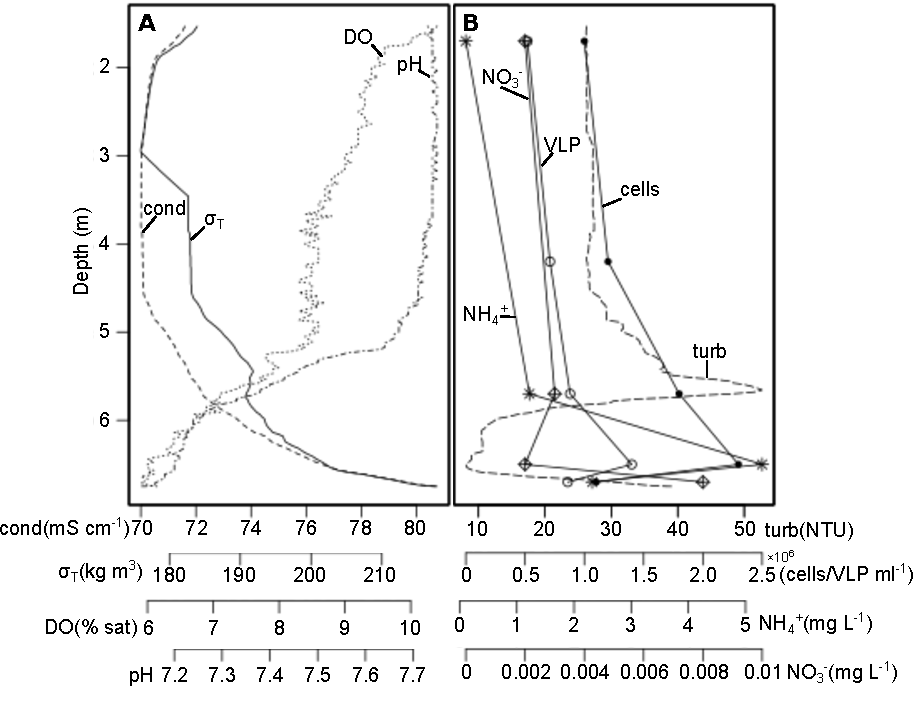
\includegraphics{orglake_figures/vert_struc.pdf}
\caption[Vertical structure of Organic Lake]{Vertical structure of Organic Lake. (\textbf{A}) Parameters that varied unimodally with depth showed two zones: an aerobic mixed zone above 5.7 m and a denser suboxic zone below. (\textbf{B}) Additional factors that revealed stratification within the deep zone. The peak in concentration at 6.5 m for ammonia was also observed for all other nutrients assayed except nitrate and nitrite, see \tabref{tab:physico-chem} for these values. $\sigma_{T} =$ (1000 $-$ density); cond, conductivity; \textsc{DO}, dissolved oxygen; turb, turbidity.}
\label{fig:vert_struc}

\end{figure}
